\begin{figure}[t]
  \centering
  \vspace{2mm}
  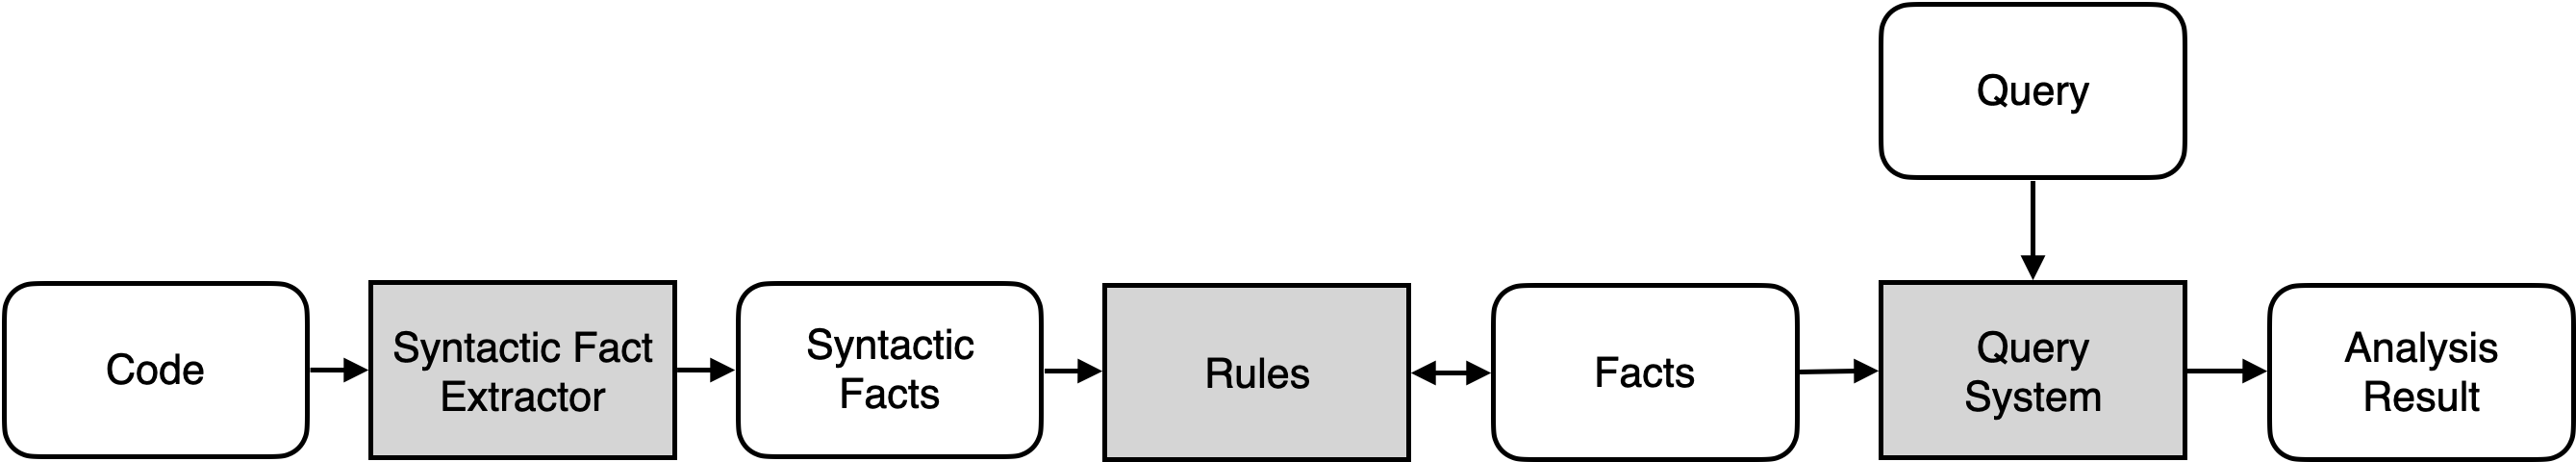
\includegraphics[width=0.94\textwidth]{img/ov1.png}
%  \vspace*{-1.5em}
  \caption{Declarative analysis for monolingual programs}
  \label{fig:ov1}
%\vspace*{-.5em}
\end{figure}

%\section{Multilingual Program Analysis using Declarative Static Analyzers}
\section{Extension of declarative style analysis for multilingual programs}
\label{sec:approach}

In this section, we propose a general approach to extend a declarative
static analysis for multilingual programs.

\subsection{Declarative Analysis for a Single Language}

%A declarative analysis~\cite{doop} consists of facts and rules, and queries:
%\[
%  \begin{array}{llll}
%f & ::= & p(\overline{elem | x}) & \mbox{fact}\\
%r & ::= & f\ \mbox{:-}\ \overline{\neg^? f} & \mbox{rule}\\
%q & ::= & \mbox{?-} \overline{f}\ &  \mbox{query}
%\end{array}
%\]
%A fact ``$f = p(\overline{elem | x})$'' denotes a relation $p$
%between elements $\overline{elem}$ or variables $\overline{x}$.
%A rule ``$r = f'\ \mbox{:-}\ \overline{\neg^? f}$'' denotes that
%a fact $f'$ can be derived from other facts $\overline{f}$;
%$f'$ holds if all the facts $d \in \{\overline{\neg^? f}\}$ hold
%and all the facts $\neg d \in \{\overline{\neg^? d}\}$ does not hold.
%A query ``$\mbox{?-} \overline{f}$'' outputs all possible mappings from
%variables to elements, such that it will make all facts in $\overline{f}$ hold.
%
%Figure~\ref{fig:ov1} presents the overview of how a
%declarative-style analysis works for monolingual programs.
%The analysis consists of three steps.
%First, a given program gets converted into database of syntactic facts.
%Second, the rules that generate new facts are defined, and
%a declarative language engine evaluates the rules with the given facts,
%producing new facts.
%Finally, the query is executed to extract all the facts that meet
%certain conditions, which correspond to the analysis result.

\medskip
\textbf{Step 1: Extracting syntactic facts.}
The first step is to extract syntactic facts from a given source code.
Syntactic facts include facts about certain AST nodes and
the parent-child relationship between nodes. For example, consider
the following code:

\begin{lstlisting}[style=cpp,xleftmargin=2.5em]
function f() {
  return 42;
}
\end{lstlisting}
We can define a syntactic fact of the form ``\datalog{functionAt(l, name)},''
where \datalog{l} denotes the line number and \datalog{name}
denotes a name of the function defined at line \datalog{l}.
Therefore, we can extract the fact \datalog{functionAt(1, "f")}/
Another example syntactic fact is ``\datalog{enclosingStmt(l1, l2, i)},''
which denotes that the function at line \datalog{l1} has the statement
at line \datalog{l2} as the \datalog{i}-th subexpression.
For example, we can extract the following syntactic facts:
\datalog{enclosingStmt(1, 2, 0)}.

In a sense, these syntactic facts serve as building blocks for the
common Intermediate Representation (IR) of multiple languages.
Compared to other IRs, this declarative-style IR has a few advantages.
First, extracting information from source code in this format does not
require any consideration of the language semantics, which imposes
almost no performance overhead beyond parsing the source code.
Second, the syntactic facts can be utilized easily in any other kind of
analysis, since they are simple information that can be freely
manipulated by defining new rules. Therefore, even when we use a different
client analysis, we can reuse the extracted syntactic facts
without re-extracting them from the source code.


\medskip
\textbf{Step 2: Defining rules.}
The next step is to define rules to generate new facts out of known facts.
%This step corresponds to actually implementing the algorithm of a
%static analysis in a declarative style.
For example, recall that we can define a call graph
\datalog{callEdge(l1, l2)} using the facts
named \datalog{functionAt} and \datalog{callAt}.
The defined rules are evaluated with declarative engines to finding all possible
facts that can be derived. The rules are usually evaluated in a bottom-up
and modular manner. Each rule is evaluated one-by-one, after every
rule it depends on is evaluated. 

\textbf{Step 3: Performing queries.}
The final step is to perform queries via query system.
The result of the query corresponds to actual result of client analysis.
A query consists of set of facts, where some of the facts would have
varaibles as arguments. Given a query, the query sytem will find all possible
assignment on variables, that will make every facts would hold under
the assignment.

\begin{figure}[t]
  \centering
  \vspace{2mm}
  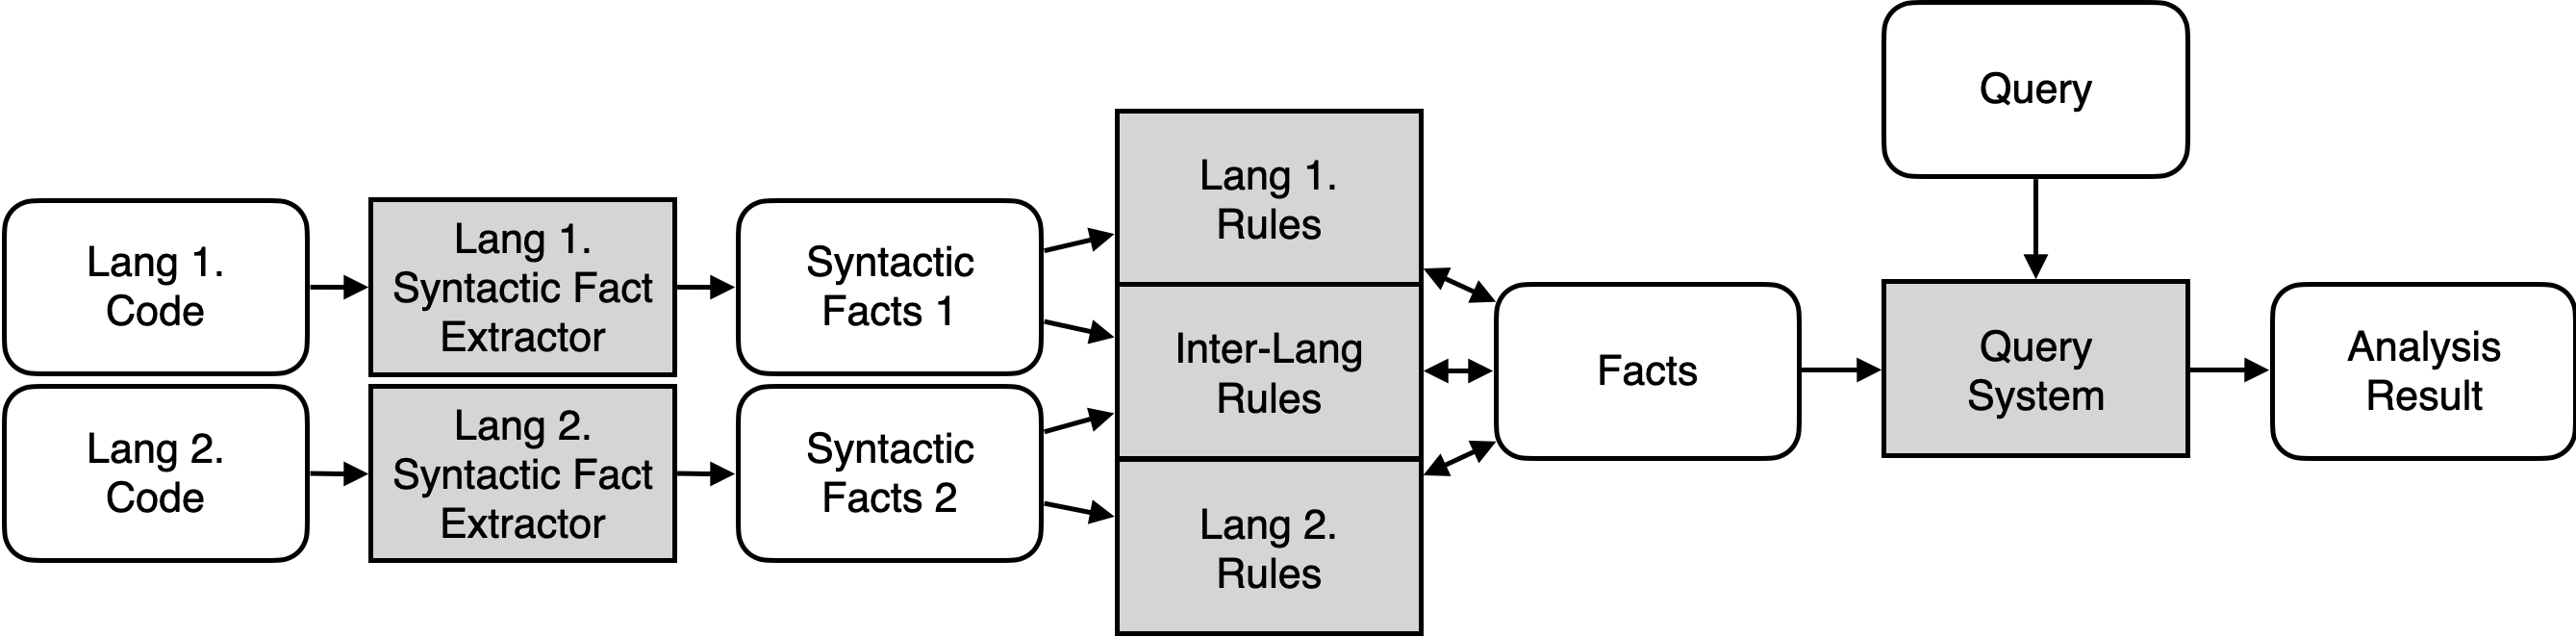
\includegraphics[width=0.94\textwidth]{img/ov2.png}
  \caption{Declarative analysis for multilingual programs}
  \label{fig:ov2}
%\vspace*{-.5em}
\end{figure}

\subsection{\mbox{Declarative Analysis for Multiple Languages}}
Now, we explain how we can compose two declarative-style static analyzers
for monolingual programs to perform analysis on multilingual programs.

Figure~\ref{fig:ov2} illustrates how we support multilingual
analysis in a declarative style in the case of two languages as an
example. The declarative language engine now gets two sets of
syntactic facts extracted from different languages. In addition,
new language-interoperation rules are defined on top of the original
language-specific rules from different languages to take the
interoperation semantics into account. Then, the same query is performed
to get the actual analysis.

%Let us revisit the dataflow analysis example for multilingual programs
%written in the language A and the language B.
%First, we merge each set of rules from each language.
%For example, we merge the rules for the fact \datalog{step} from each language:
%\begin{lstlisting}[style=myDatalog,xleftmargin=2.5em]
%step(a, b) :- step_A(a, b)
%step(a, b) :- step_B(a, b)
%\end{lstlisting}
%To take inter-language dataflows into account, we should also specify
%how a data of one language can be passed to another language cross language
%boundaries.  For example, one can pass data in one language into
%another by a function call as shown below:
%
%\begin{lstlisting}[style=java,xleftmargin=2.5em]
%public void main() { // Language A
%  int x = SOURCE();
%  B::f(x);
%}
%void f(int param) {  // Language B
%  printf("\%d", param);
%}
%\end{lstlisting}
%The variable \javacode{x} in the language A is passed to the parameter
%of a function \javacode{f} in the language B.  To reflect such a data flow,
%we can define the fact \datalog{foreignArgParam(a, b, i)},
%which denotes that \datalog{a} is the \datalog{i}-th argument of a foreign
%function call to a function whose \datalog{i}-th parameter is \datalog{b}.
%From the above example, we can derive the fact \datalog{foreignArgParam(x, param, 0)}.
%Using this fact, we can add a new rule to derive the common fact
%\datalog{step} as follows:
%\begin{lstlisting}[style=myDatalog,xleftmargin=2.5em]
%step(a, b) :- foreignArgParam(a, b, i)
%\end{lstlisting}
%which enables dataflows via foreign function calls cross language boundaries.
